
\part{Questions de recherche et méthodologie}

\chapter{L’évolution de nos préférences psychologiques, un paradigme évolutionnaire}

\section{Les fondements de la psychologie évolutive}

Comme pressenti plus haut, le pouvoir explicatif des grands mouvements culturels appliqués aux changements dans la psychologie et le comportement des individus peut paraitre assez limité. En l’occurrence, l'idée qu'avec la montée de l'individualisme, appréhendé comme une évolution culturelle \textit{sui generis}, chaque individu aurait tendance à devenir de plus en plus égocentrique, contribuant ainsi à enraciner l'avènement de cette nouvelle ère du « je » au niveau collectif (qui n’existe en réalité que par la somme de ses membres) frustre par son apparente circularité.

Le paradigme évolutionnaire constitue ainsi une explication alternative intéressante, où l'Histoire est bien celle des individus avant d’être celle du groupe. Selon lui, notre plasticité adaptative, définie comme la capacité à moduler notre phénotype (à savoir l'ensemble de nos caractéristiques observables) en fonction de l'environnement, impliquerait notamment la modulation de nos préférences psychologiques. Ces changements psychologiques seraient les mécanismes « proximaux » permettant \textit{in fine} à chaque individu d'optimiser sa stratégie d'allocation des ressources en fonction des transformations de son milieu (cette stratégie constituant le mécanisme « ultime » dans l'optimisation de son succès reproductif individuel).

Car le phénotype optimal d'un individu, qui inclut, outre ses caractères physiques, ses stratégies comportementales, traits de personnalité et préférences psychologiques, varie de fait en fonction des ressources disponibles dans son environnement, entendues au sens large (matérielles, institutionnelles, etc). En particulier, les modèles d'allocation optimale des ressources montrent que les individus devraient investir dans les besoins dont le rendement marginal est le plus élevé. Et étant donné que les besoins ont des rendements marginaux décroissants, lorsque les individus ont plus de ressources à investir, ils commenceraient à allouer des ressources à de nouveaux besoins. A mesure que les individus progressent dans la pyramide des besoins\footnote{\cite{maslow_theory_1943}}, leur psychologie se modifierait, et ils développeraint des préférences leur permettant, ultimement, de tendre vers la satisfaction des besoins devenus les plus adaptatifs dans l'environnement considéré (à savoir ceux qui maximisent leur \textit{fitness}, qui constitue la représentation quantitative du succès reproductif de l'individu).

\begin{figure}[!ht]
    \centering
    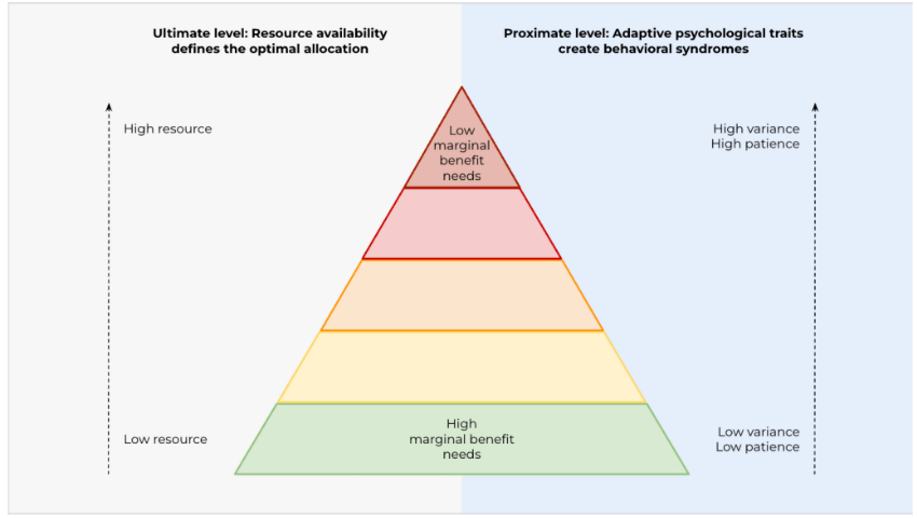
\includegraphics[width=17cm]{img/pyramide_besoins.png}
    \caption{La Pyramide des besoins de Maslow (1943) intégrée à un paradigme évolutionnaire}
    \label{pyramide_besoins}
\end{figure}

À cet égard, et en ce qui concerne l'agentivité, au fur et à mesure que l'environnement devient plus riche et plus prévisible, il deviendrait de plus en plus adaptatif pour un individu de se penser comme capable d'avoir une prise sur le monde extérieur, précisément parce que l'autonomie devient alors possible, et que les efforts investis sont susceptibles de générer des bénéfices individuels additionnels. A l'inverse, dans un environnement très incertain et/ou hostile, il serait plus adaptatif de se sentir relativement moins agentif et de préférer s'en remettre à l'apprentissage de lois extérieures alors perçues comme « naturelles ». Cela permettrait en effet de s'en accommoder au mieux, puisqu'il serait \textit{de facto} plus difficile, voire impossible, d’infléchir ces forces extérieures en faveur de projets autonomes, ces derniers représentant alors un effort relativement vain, voire désavantageux en termes de fitness.

Autant de considérations qui font écho au compromis de Vallacher\footnote{\cite{vallacher_levels_1989}} mentionné précédemment, mais formulé cette fois en des termes évolutionnaires : lorsque la quantité de ressources dans l'environnement est suffisamment élevée pour que la plupart des actions réalisées soient relativement faciles à prendre en charge (y compris la possibilité de s'appuyer sur un système institutionnel pour déléguer une partie de la satisfaction de ses besoins « les plus bas »), l'individu n'aurait plus besoin de s'attarder sur leurs détails mécaniques, et pourrait se permettre d'allouer ses ressources cognitives à l’interprétation plus abstraite de ses actions, le développement de capacités de planification associées étant susceptible d'optimiser son succès reproductif à plus long terme. 

De tout ce qui précède, deux questions de recherche se posent pour nous, dont seule la première sera abordée dans le cadre de ce mémoire : 

1. Est-il possible de construire un indice linguistique d'agentivité, c'est-à-dire un faisceau de marqueurs linguistiques qui permette de mesurer le degré d'agentivité d'un texte, et par extension, de son locuteur ?

2. Si tel est le cas, comment l’agentivité, mesurée par un tel indice, varie-t-elle avec le temps et les ressources dans une société donnée ? Sur la base du paradigme adopté, nous supposons que le niveau « moyen » d’agentivité dans une société devrait être positivement corrélé avec son niveau de ressources.

\section{Les fictions narratives, des « produits dérivés » de l’esprit humain}

Si notre ambition ultime est celle d’exploiter notre indice linguistique pour retracer l’évolution de l’agentivité d’individus réels, pourquoi donc l’élaborer à partir de textes fictionnels ? Il se trouve que notre paradigme évolutionnaire fait de la fiction narrative un support particulièrement pertinent pour retracer l'histoire de la psychologie humaine. 

De fait, il est possible de considérer les fictions narratives comme des « produits dérivés » de l'esprit humain, à savoir qu'elles n'auraient pas évolué par sélection naturelle mais auraient coopté certaines préférences et mécanismes cognitifs préexistants, sélectionnés avant même l'émergence de la culture symbolique et pour d'autres raisons liées à notre Environnement d'Adaptation Évolutive (l'environnement ancestral auquel notre espèce est adaptée)\footnote{\cite{dubourg_why_2022}}. Selon cette hypothèse, la fiction survit car nous tirons certains bénéfices de la production et de la consommation de ces objets culturels attrayants, ce qui la rend indirectement adaptative.

Les fictions narratives peuvent ainsi être considérées comme des « technologies de divertissement », à savoir comme des objets conçus par certaines personnes dans le but immédiat d'attirer l'attention des autres, et dans le but ultime de remplir d'autres fonctions évolutives pertinentes qui deviennent plus faciles à atteindre une fois que l'attention des autres a été captée. Cela permettrait d'expliquer pourquoi la fiction est souvent remplie de stimuli exagérés et divertissants, pourquoi elle s'adapte si bien aux préférences changeantes du public qu'elle cible, et pourquoi les producteurs rendent leur fiction de plus en plus attrayante au fil du temps, ce de manière cumulative.

Les fictions peuvent donc servir de miroir pour retracer l'évolution dans le temps de ces préférences psychologiques que chaque lecteur dicte et que chaque auteur coopte, et qui changent en fonction des transformations du milieu.

\chapter{Construction d’un indice d’agentivité global : une approche par faisceau d’indices}

\section{Validation interne : le choix d’un corpus théâtral}

Se pose alors la question du corpus à sélectionner pour éprouver notre indice agentif, dont nous détaillerons la composition dans la partie suivante. Les indicateurs linguistiques ayant été choisis sur la base de la langue française, l'étude porte ici sur les productions littéraires françaises.

En particulier, la forme stylistique relativement standardisée du théâtre permet de contrôler certaines variations qui pourraient être liées à des phénomènes plus aléatoires de transmission culturelle plutôt qu'à la sélection et à la plasticité proprement dites, qui font du passage d'une préférence psychologique à une autre la réponse spécifique et optimale à certains changements environnementaux, préférence qui se refléterait en partie dans le choix des mots.

Le genre théâtral présente également l'avantage de disposer de corpus substantiels déjà constitués et librement accessibles en ligne. En l'occurrence, nous avons choisi de retenir le corpus de théâtre classique librement téléchargeable sur le site \small{\url{www.theatre-classique.fr}}, comprenant les principales œuvres théâtrales publiées en France entre 1550 et 1800.

Surtout, la dualité théâtrale classique entre personnages maîtres et serviteurs fournit un critère de validation interne particulièrement solide pour notre indice agentif. Par définition, il semble en effet raisonnable de considérer que les maîtres sont relativement plus agentifs que leurs serviteurs. Il s’agira alors de comparer le score global de l'indice obtenu pour les répliques prononcées par tous les personnages maitres et serviteurs respectivement, une première étape pour tester la capacité de l’indice à tracer \textit{quelque chose comme l'agentivité} dans un texte.

Concrètement, nous avons attribué à chaque personnage des pièces étudiées un statut sur la base des mots-clés apparaissant ou non pour le décrire dans la didascalie de chaque pièce. Pour considérer un personnage comme « serviteur », ou plutôt comme doté d’un « bas statut » (le terme de « serviteur » est entendu ici dans un sens générique), statut pour lequel les mentions dans la didascalie étaient les moins ambiguës, nous avons retenu les mots-clés suivants : « domestique », « esclave », « chambre » (pour « femme de chambre »), « camariste », « servant », « servante », « suivante », « valet », « suite », « confident », « confidente ». Notons que nous avions accès à une liste de tous les « rôles » pris par les personnages dans l'ensemble du corpus, référencée par le site mentionné ci-dessus. C'est à partir de cette liste que nous avons construit notre liste de mots-clés, qui se trouve donc être exhaustive pour ce corpus.

Pour les personnages dits « haut statut », dont les mentions étaient parfois ambiguës ou simplement trop variées pour procéder par liste de mots-clés malgré l'existence d'un tel référencement, nous avons retenu la règle suivante : tout personnage dont le nom X apparaît en complément d'un mot-clé « bas statut » (par exemple « valet de X ») est automatiquement considéré comme appartenant au groupe « haut statut », dans le sens où il a quelqu'un à son service. Cela semblait être la manière la plus neutre et la plus pertinente de procéder, sans être soumis aux variations socio-historiques dont pourrait souffrir le sens d'étiquettes telles que « bourgeois », et en relation avec notre concept d'agentivité - l'idée étant qu'un personnage capable d'en commander un autre est \textit{a fortiori} plus agentif que celui qu'il ou elle commande. Pour chaque pièce considérée, les répliques des personnages qui ne répondaient pas à ces critères dans la didascalie, et n’appartenaient donc à aucun des deux groupes, ont été exclues de l'analyse linguistique.

A partir de là, nous avons codé une manière d'attribuer à chaque personnage inclus dans l’analyse les répliques qu'il ou elle formulait dans l'ensemble de la pièce. Nous avons ensuite concaténé l’ensemble des répliques respectivement prononcées par des personnages « bas » et « haut » statut, afin de pouvoir comparer leur score agentif au niveau de chaque pièce.

\section{Validation externe : plusieurs propositions}

Nous avions également besoin d’une validation externe de notre indice, afin de s’assurer qu’il trace l’agentivité spécifiquement, sans être corrélé à d'autres dimensions psychologiques telles que la communion, auquel cas il ne saurait être informatif.

À cette fin, il existe tout d’abord une vaste littérature établissant un lien entre agentivité et masculinité\footnote{\cite{neria_encyclopedia_2016}}. Examiner en parallèle si l'indice est préférentiellement corrélé avec les répliques de personnages masculins plutôt que féminins était ainsi une première façon de s'assurer de la spécificité de sa mesure.

En outre, il nous a semblé utile de comparer notre indice avec des marqueurs linguistiques spécifiques d’autres dimensions psychologiques, pour lesquelles nous ne nous attendions pas à des corrélations avec le statut du personnage, et par conséquent avec l'indice agentif. Malheureusement, aucune étude à ce jour ne s'est intéressée aux corrélations potentielles entre la communion, \textit{a priori} orthogonale à l’agentivité, et certains marqueurs linguistiques, ce qui suffirait à faire l'objet d'un projet de recherche à part entière. 

Il a donc fallu se tourner à nouveau vers le modèle des \textit{Big 5}, en dépit de ses limites. Il se trouve en effet que certains des cinq traits qui le composent entretiennent une relation privilégiée avec les deux dimensions supérieures que sont l’agentivité et la communion. 

Pour l'observer, il faut en réalité mobiliser, outre les modèles dimensionnels comme celui des \textit{Big Five}, la notion de circomplexes. Egalement très utilisés en psychologie pour décrire les relations entre un ensemble de variables, les modèles circomplexes sont généralement définis en termes de corrélations systématiques croissantes et décroissantes entre les variables, et peuvent être représentés visuellement sous la forme d'un cercle dans lequel les variables adjacentes sont fortement corrélées et les variables opposées sont inversement corrélées. Ils ont notamment été utilisés pour décrire les dispositions interpersonnelles\footnote{\cite{wiggins 1979}}. 

A partir d’un échantillon de 315 hommes et femmes adultes, et en factorisant conjointement les auto-évaluations passées sur les Échelles d'Adjectivité Interpersonnelle révisées de Wiggins\footnote{Le comportement interpersonnel ayant souvent été caractérisé par des modèles circumplexes, Wiggins a entrepris de créer un ensemble d'échelles adjectives présentant des propriétés circumplexes, et auxquelles on se réfère ici. Voir \cite{wiggins_psychological_1979}} avec des auto-évaluations, des évaluations par les pairs et des évaluations par le conjoint fondées sur l'Inventaire de Personnalité NEO\footnote{Le NEO-PI est un questionnaire de 181 items développé pour opérationnaliser le modèle à cinq facteurs. Les réponses aux items du NEO-PI se font sur une échelle de Likert en 5 points. Une forme à la troisième personne du NEO-PI a également été mise au point et validée pour être utilisée par des évaluateurs. \cite{costa 1985}}, ce afin d'examiner les relations entre les deux modèles, McCrae et Costa\cite{mccrae_structure_1989} ont pu constater que le circomplexe interpersonnel était défini par les deux dimensions que sont l'extraversion et l'agréabilité.

\begin{figure}[!ht]
    \centering
    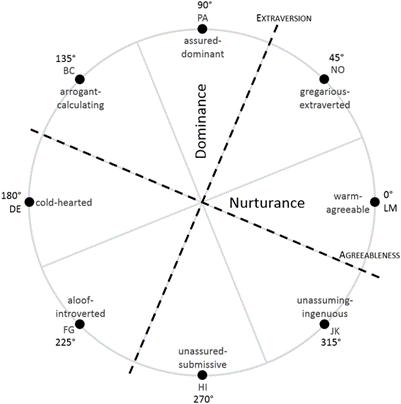
\includegraphics[width=12cm]{img/circumplex_wiggins.png}
    \caption{Le Circomplexe interpersonnel de Wiggins (1995) et le Modèle à 5 facteurs ou \textit{Big Five}}
    \label{circumplex_wiggins}
\end{figure}
\newpage


Comme apparent sur le cercle, les axes de l'agréabilité et de l'extraversion du \textit{Big Five} sont en effet situés à environ 45 degrés des axes familiers de l'amour et du statut de ce circomplexe, et semblent donc traiter d'aspects différents des mêmes dimensions latentes. A titre de remarque, l'extraversion est définie dans le modèle des \textit{Big Five} comme une activité tournée vers l'extérieur, mais non comme un « comportement prosocial » (elle ne décrit pas, par exemple, à quel point une personne se soucie sincèrement des autres). C'est l'agréabilité qui fait précisément office de liant social, caractérisant quant à elle des personnes plus tolérantes, douces, indulgentes, agréables, altruistes et obligeantes. 

L'agréabilité et l'extraversion se rapporteraient ainsi plus étroitement au comportement interpersonnel que les mesures des domaines restants du NEO-PI (névrosisme, conscienciosité et ouverture à l'expérience). Pour autant, nous avons également inclus dans les traits de personnalité préférentiellement associés à l’agentivité qui nous intéressent ici la conscienciosité, sur la base d’un certain nombre de travaux plus récents\footnote{\cite{hurley_agency_1998}\footnote{\cite{abele_facets_2016} - en notant que dans cette étude et en dépit de la définition retenue dans le \textit{Big Five}, l'extraversion est également associée à la Communion. Cela rend donc l'ajout la consciensioté plus pertinent encore, afin que notre méthode de validation externe ait toutes les chances d'être concluante}}. De la même façon, outre l'agréabilité, l'ouverture y est parfois positivement corrélée avec la communion, et est donc également prise en compte dans notre étude.

\section{Outils utilisés}

Bien que nous détaillions de manière exhaustive les composantes de l’indice global d’agentivité dans le chapitre suivant, elles sont récapitulées et réparties ici dans des catégories définies sur la base des différentes facettes du concept d’agentivité mentionnées plus tôt, et qui ont pour partie inspiré la sélection de ces différents éléments linguistiques supposés avoir trait à l’agentivité :  

\begin{center}
\begin{table}[ht]
\caption{Récapitulatif des marqueurs linguistiques retenus}
\bigskip
\renewcommand{\arraystretch}{1.5} % Adjust the value as needed
\begin{tabular}{ |p{3cm}|p{3cm}|p{3cm}|p{3cm}|p{3cm}|p{3cm}| }
 \hline
 \textbf{Sentiment d'agentivité} \newline{Locus de Contrôle} &  \textbf{Efficacité de l'action*} \newline{Disposition objective à l'action} & \textbf{Volition} \newline{Degré de connotation agentive des évènements décrits} & \textbf{Identification à l'action} \newline{Degré de référence à soi} & \textbf{Compréhension globale} \newline{Capacité de distanciation psychologique}  \\
 \hline
 \textit{Verbes} &  Agentivité grammaticale (orateur-sujet) & Transitivité & Pronoms (individuels vs. collectifs, à la 1ère personne) & Modes irréels \\
    Voix active vs. passive & \textit{Verbes} & Télicité & Déictiques (proximaux vs. distaux) & Alternance de temps \\
    Modalité (interne vs. externe) & Evènements vs. états & Adverbes intentionnels & & Degré d'abstraction (adverbes, mots-outils, adjectifs)\\
 \hline
\end{tabular}
\end{table}
    \label{recap_marqueurs_agentifs}
\end{center}
\vspace{-20pt} % Adjust the value to reduce the space
\textit{* L’agentivité telle que nous la comprenons, et contrairement à Hopper et Thompson\footnote{\cite{hopper_transitivity_1980}}, ne semble pas impliquer l'accomplissement le plus total de l'action, et/ou l'affectation la plus complète de l'objet s'il y en a un, mais plutôt la possibilité (le « pouvoir » de l'agent) et l'actualité d'une telle action (le fait qu'il y ait une action évoquée, plutôt qu'un état), ces deux concepts définissant l'efficacité de l'action, à laquelle l’agentivité ne saurait par ailleurs se réduire.}


Dans le tableau ci-dessus, la direction prédite est toujours positive, à savoir que chaque indicateur est supposé être positivement corrélé avec le niveau d’agentivité du personnage locuteur. En italique sont mentionnés les indicateurs pour lesquels la direction est ambigüe. La mention « vs.» signifie que la métrique consiste en un ratio entre les deux notions mises en rapport (calculé dans l'ordre d'apparition de ces dernières). Par exemple, la métrique « Voix active vs. passive » est égale au ratio (nombre d'occurrences de la voix active)/(nombre d'occurrences de la voix passive). Enfin, lorsque cette mention « vs. » apparait entre parenthèses, cela signifie qu'une métrique existe également pour compter le nombre total d'occurrences du marqueur en question (en plus du ratio mentionné). A titre d'exemple, notre indice agentif inclut à la fois une métrique calculant la fréquence totale des déictiques dans les répliques étudiées, et une métrique calculant le ratio (nombre de déictiques proximaux)/(nombre de déictiques distaux) dans ces dernières.

Concernant l’analyse textuelle, nous avons utilisé le modèle \textit{fr-dep-news-trf} de spaCy\footnote{\url{https://spacy.io/}}, ainsi que le modèle \textit{fr} de pie-extended\footnote{\url{https://github.com/hipster-philology/nlp-pie-taggers}}. Chacun des marqueurs linguistiques a été normalisé en fonction du nombre total de mots prononcés respectivement par les personnages haut et bas statut, dans chaque pièce, à l'exception : 

-des signes de ponctuation individuels (rapportés à la ponctuation totale) ; 

-des verbes conjugués (cette métrique, ainsi que celle mesurant le gérondif spécifiquement), modaux, transitifs, « statifs » et copules, des verbes dont le sujet est à la première personne et des marqueurs de négation (rapportés au nombre total de verbes) ; 

-des métriques de temps et modes (subjonctif etc) (rapportées au nombre total de verbes conjugués)

-du marqueur d’agentivité grammaticale (rapportée au nombre total de phrases) ;

-des duplicata d’indicateurs pour lesquels la contrainte d’avoir un sujet à la première personne nous semblait pertinente à ajouter (rapportés au nombre total de verbes ayant un sujet à la première personne) 

-et des ratios, a fortiori.
